% !TeX spellcheck = en_US
\documentclass[letterpaper,12pt,twoside]{report}
\usepackage{fancyhdr}
\usepackage{fullpage}
\usepackage{tikz}
\usepackage{amsmath}

\begin{document}
	\pagestyle{fancy}
	\fancyhf{}
	\fancyhead[L]{Day 16}
	\fancyhead[R]{\textit{The Calendar Project}}
	\fancyfoot[L]{Citations Involved: none}
	
	% Problem
	\paragraph{Problem}
	\begin{quote}
		\textsf{Find the minimum distance that
			connects the points $A(0, y)$, $B(2, -1)$,
			$C(x, 7)$, and $D(5, 4)$ in the
			order $A$-$B$-$C$-$D$.}
	\end{quote}
	
	% Graphics
	\begin{center}
		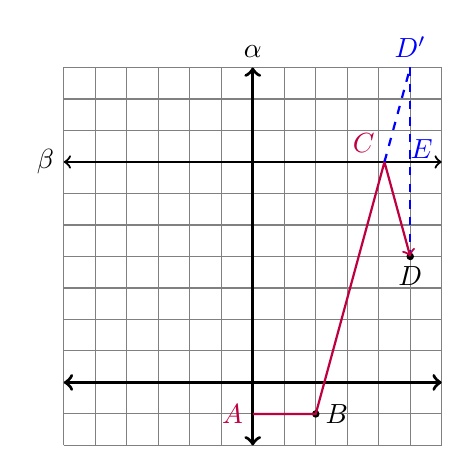
\begin{tikzpicture}[scale=0.4]
		\draw[gray, thin] (-6,-2) grid (6,10);
		\draw[<->,very thick] (6,0) -- (-6,0);
		\node[left] at (-6,7) {$\beta$};
		\draw[<->,very thick] (0,-2) -- (0,10);
		\node[above] at (0,10) {$\alpha$};
		
		\draw[fill] (2,-1) circle [radius=0.1];
		\node[right] at (2,-1) {$B$};
		\draw[fill] (5,4) circle [radius=0.1];
		\node[below] at (5,4) {$D$};
		\draw[blue,dashed,thick] (5,10) -- (5,4);
		\node[above right,blue] at (4.7,6.8) {$E$};
		\draw[<->,thick] (-6,7) -- (6,7);
		\node[above left,purple] at ({46/11},7) {$C$};
		\node[left,purple] at (0,-1) {$A$};
		
		\draw[->,thick,purple] (0,-1) -- (2,-1) -- ({46/11},7) -- (5,4);
		\draw[blue,dashed,thick] ({46/11},7) -- (5,10);
		\node[above,blue] at (5,10) {$D^\prime$};
		
		\end{tikzpicture}
	\end{center}
	
	\textit{Note: This problem is being interpreted such that $x$ and $y$ refer to real values that minimize the distance being queried.}
	% Reasoning
	\paragraph{Reasoning}
	\begin{quotation}
		
		The only information given about $A$ is that its $x$ component is equal to 0; its $y$ component is unknown, so the locus of all possible points that satisfy the given constraint is the line with equation $x=0$; name this line $\alpha$. The only information given about $C$ is that its $y$ component is equal to 7; its $x$ component is unknown, so the locus of all possible points that satisfy the given constraint is the line with equation $y=7$; name this line $\beta$.
		
		The distance from a point to a line is the length of the perpendicular segment from the point to the line (4). Since the equation $x=0$ of $\alpha$ has an undefined slope, the slope of a line perpendicular to it is 0. With a slope and a point through which the line containing $\overline{AB}$ passes, $\overleftrightarrow{AB}$'s equation can be expressed in point-slope form and then converted into slope-intercept form: $y-(-1)=0(x-2) \Rightarrow y+1=0 \Rightarrow y=-1$. The point of intersection between this line and $\alpha$ is derived from their equations ($x=0, y=-1$) to be $(0,-1)$. These are the coordinates of $A$ such that $\overline{AB}\bot\alpha$. Thus established, $AB$ is the distance from $B$ to $\alpha$. By the Distance Formula, $AB=\sqrt{(2-0)^2+(-1-(-1))^2}=\sqrt{4}=2$.
		
		Reflect $D$ across $\beta$ and name the image $D^\prime$. Since the pre-image and the image are equidistant from the line of reflection (3), $CD=CD^\prime$. By the SAP, $BD^\prime=BC+CD^\prime$; after substitution, $BD^\prime=BC+CD$. Since the  minimum distance between two points is that of the segment connecting them, the minimized value of $BC+CD$ given the coordinates of $B$, coordinates of $D$, and the constraint of $y=7$ for $C$ is $BD^\prime$. 
		
		Since the line of reflection is the perpendicular bisector of each segment joining each point and its image (5), $\beta$ bisects $\overline{DD^\prime}$ and $\beta\bot\overline{DD^\prime}$. $\beta$'s equation is $y=7\Rightarrow y=0x+7$, meaning that the slope of $\beta$ is 0. The perpendicular slope of $\beta$ is the negative reciprocal of 0, or $-\frac{1}{0}=\text{undefined}$, meaning that $\overleftrightarrow{DD^\prime}$ is a vertical line. With its slope and a point through which it passes known, $\overleftrightarrow{DD^\prime}$ can be expressed as the equation $x=5$. Name $E$ as the intersection between $\overleftrightarrow{DD^\prime}$ and $\beta$. The coordinates of $E$ are determined by combining the equations for $\beta$ and $\overleftrightarrow{DD^\prime}$, $y=7$ and $x=5$, to produce $E(5,7)$. Since $\beta$ bisects $\overline{DD^\prime}$, $E$ is the midpoint of $\overline{DD^\prime}$. Let $D^\prime$ have coordinates $(x_{D^\prime}, y_{D^\prime})$. By the Midpoint Formula (1), $(\frac{5+x_{D^\prime}}{2},\frac{4+y_{D^\prime}}{2})=(5,7) \Rightarrow \frac{5+x_{D^\prime}}{2} = 5, \frac{4+y_{D^\prime}}{2}=7 \Rightarrow 5+x_{D^\prime}=5\cdot2=10, 4+y_{D^\prime}=7\cdot2=14 \Rightarrow x_{D^\prime}=10-5=5, y_{D^\prime}=14-4=10$. Therefore $D^\prime$ has coordinates $(5,10)$. By the Distance Formula (2), $BD^\prime=\sqrt{(5-2)^2+(10-(-1))^2}=\sqrt{3^2+11^2}=\sqrt{130}$. Having deduced previously that $BD^\prime=BC+CD$, $BC+CD=\sqrt{130}$ by the Transitive Property.
		
		The distance being queried in the problem can be represented by $AB+BC+CD$. After substitution, $AB+BC+CD=2+(BC+CD)=\boxed{2+\sqrt{130} \text{  units}}$.
				
	\end{quotation}
	
	\paragraph{External References}
	
	\begin{enumerate}
		\item Textbook Ch. 1, Pg. 43: Midpoint Formula
		\item Textbook Ch. 1, Pg. 44: Distance Formula
		\item Textbook Ch. 1, Pg. 50: Transformations
		\item Textbook Ch. 3, Pg. 172: Definition of the Distance from a Point to a Line
		\item Textbook Ch. 12, Pg. 825: Reflections
	\end{enumerate}
	
\end{document}